
\chapter{Experimentos} \label{cap:experimentos}


% [objetivo]

En este capítulo hacemos una comparación empírica entre $\BiasPMI$ y $\BiasWE$ a fin de ilustrar las principales diferencias entre las métricas. En particular, nos proponemos comparar los métodos en las siguientes tres dimensiones:

\begin{itemize}
    
    \item \textbf{Variabilidad:} ¿Cómo difieren los métodos de medición de la variabilidad de $\BiasPMI$ y $\BiasWE$? (sección \ref{sec:experimento_variabilidad})
    
    \item \textbf{Correlación con el juicio humano:} ¿En qué medida las estimaciones de $\BiasPMI$ y $\BiasWE$ correlacionan con el juicio humano de los sesgos? (sección \ref{sec:experimento_correlacion})

    \item \textbf{Interpretabilidad:} ¿Qué tipos de asociaciones semánticas capturan $\BiasPMI$ y $\BiasWE$? (sección \ref{sec:experimento_interpretabilidad})

\end{itemize}


\section{Aspectos metodológicos} \label{sec:metodologia}

\subsection{Corpus} \label{sec:corpus}

Para los experimentos usamos un \emph{corpus} en inglés construido a partir de \textbf{\emph{English Wikipedia}} de agosto de 2014 (\url{https://archive.org/download/enwiki-20141208}) al que llamamos, de aquí en más, Wikipedia. 

% OpenSubtitles (TODO ref Lison y Tiedemann, 2016), que consiste en subtítulos en inglés de películas y programas de televisión y construimos con la ayuda de la librería de Python subs2vec (van Paridon y Thompson, 2021). 

En el \textbf{preprocesamiento} se eliminan los artículos con menos de 50 tokens, se convierten los tokens a minúsculas, se eliminan los símbolos no alfanuméricos y se aplica una partición en oraciones (\emph{sentence splitting}), de modo que una oración equivalga a un documento. Tras aplicar estos pasos, el corpus de Wikipedia consta de 1.200 millones de tokens y 53,9 millones de documentos. 

% mientras que el de OpenSubtitles contiene 2.400 millones de tokens y 447,9 millones de documentos.

\subsection{Medición de sesgos}

Para cuantificar los \textbf{sesgos textuales}, computamos $\BiasWE$ usando SGNS, FastText y GloVe según la ecuación \ref{eq:bias_we}, mientras que usamos la ecuación \ref{eq:bias_pmi_estimado} para $\BiasPMI$. 

Nos enfocamos en medir sesgos que ya han sido estudiados por la literatura existente, la cual usamos como referencia para definir las listas de palabras de contexto $A$ y $B$. Asimismo, medimos cada uno de los sesgos en palabras objetivo cuyos \textbf{sesgos de acuerdo al juicio humano} han sido medidos por estudios previos, en experimentos independientes de la Wikipedia. De esta manera nos aseguramos de estar midiendo los sesgos en palabras donde es razonable estudiarlos en el contexto de las ciencias sociales computacionales.

En particular, medimos los siguientes sesgos:


\begin{description}[leftmargin=\parindent,labelindent=\parindent]

    \item[Sesgo de género.] Aquí \emph{A=\{female, woman, girl, sister, she, her, hers, daughter\}} y \emph{B=\{male, man, boy, brother, he, him, his, son\}} \citep{caliskan2017semantics}. Valores positivos (negativos) indican que la palabra objetivo se asocia relativamente más con los términos femeninos (masculinos). 

    Medimos el sesgo de género en las palabras de las \emph{Glasgow Norms}, un conjunto de 5.500 palabras en inglés con puntajes de género que resumen las respuestas de los participantes a los que se pidió que valoraran la asociación de género de cada palabra \citep{scott2019glasgow}. Los participantes midieron el grado en que cada palabra se asocia a un comportamiento masculino o femenino en una escala de 1 (muy femenino) a 7 (muy masculino). Siguiendo a \citet{lewis2020gender}, promediamos las normas de los homónimos y calculamos $8 - puntaje$ para invertir la escala de los puntajes de modo que representen la feminidad según el juicio humano. 4.661 palabras de la lista original coinciden con el vocabulario de Wikipedia.

    \item[Sesgo étnico.] Usamos \emph{A=\{black, blacks, african, afro\}} y \emph{B=\{white, whites, european, anglo\}} \citep{kozlowski2019geometry}. Valores positivos (negativos) indican que la palabra objetivo se asocia relativamente más con los términos de etnia negra (blanca). 

    \citet{kozlowski2019geometry} seleccionaron 60 palabras de siete ámbitos temáticos (ocupaciones, alimentos, ropa, vehículos, géneros musicales, deportes y nombres de pila) y pidieron a 398 encuestados de Amazon Mechanical Turk que valoren cómo calificarían cada palabra en una escala de 0 (\emph{very African American}) a 100 (\emph{very white}). La valoración promedio de estas respuestas representa la asociación relativa \emph{black-white} de cada palabra según el juicio humano. Medimos el sesgo étnico en las 59 palabras que coinciden con el vocabulario de nuestro \emph{corpus}.

    \item[Sesgo de sentimiento.] Aquí 
    \emph{A=\{caress, freedom, health, love, peace, cheer, friend, heaven, loyal, pleasure, diamond, gentle, honest, lucky, rainbow, diploma, gift, honor, miracle, sunrise, family, happy, laughter, paradise, vacation
    \}} 
    y 
    \emph{B=\{abuse, crash, filth, murder, sickness, accident, death, grief, poison, stink, assault, disaster, hatred, pollute, tragedy, divorce, jail, poverty, ugly, cancer, kill, rotten, vomit, agony, prison\}} 
    \citep{caliskan2017semantics}. Valores positivos (negativos) indican que una palabra objetivo se asocia relativamente más con los términos agradables (desagradables). En la bibliografía en inglés este sesgo se suele denominar \emph{valence bias} \citep{toney2021valnorm}.

    En este caso consideramos las palabras del estudio de \citet{warriner2013norms}, en el que 1.827 trabajadores de Amazon Mechanical Turk calificaron 13.915 palabras de tópicos diversos en una escala de 1 (\emph{unhappy}) a 9 (\emph{happy}). El sentimiento de cada palabra de acuerdo al juicio humano se computa como el promedio de estas calificaciones. En este trabajo medimos el sesgo de sentimiento en las 13.565 palabras que están en el vocabulario de Wikipedia.

\end{description}

% TODO Tablas con palabras?

\subsection{Detalles de implementación}

%[librerías, hiperparámetros, etc.]

En todas las metodologías utilizadas (SGNS, FastText, GloVe y PMI), contamos las coocurrencias a partir de una ventana de tamaño $\pm 10$ dentro de cada oración ($T=10$). Consideramos a los tokens con menos de 100 apariciones como OOV (fuera del vocabulario) y los eliminamos antes de computar la matriz de coocurrencias.

Para entrenar SGNS y FastText, usamos la implementación de Gensim \citep{rehurek2010gensim}, mientras que para GloVe usamos la implementación de \citet{pennington2014glove}. En los tres casos los vectores tienen 300 dimensiones y usamos los hiperparámetros por defecto. En el caso de PMI, contamos las coocurrencias con el módulo de GloVe \citep{pennington2014glove}, y establecemos el parámetro de suavizado $\epsilon$ en 0,01.

Todos los experimentos se realizaron en una máquina de escritorio con un procesador Intel Core i5-4460 de 4 núcleos a 3,20 GHz y 32 GB de RAM. 


\section{Estimación de la variabilidad} \label{sec:experimento_variabilidad}

Para cada uno de los sesgos medidos en sus respectivas palabras objetivo, calculamos el \textbf{p-valor de permutaciones} de $\BiasWE$ (10.000 permutaciones) y el \textbf{p-valor del test de log odds ratio} de $\BiasPMI$, considerando la hipótesis nula de ausencia de sesgo. Aplicamos la corrección de Benjamini-Hochberg a los p-valores de cada método de medición de sesgo por separado para ajustar por las comparaciones múltiples \citep{benjamini1995correction}. También computamos los \textbf{intervalos de confianza} de 95\% para cada estimación, usando bootstrap en el caso de $\BiasWE$ (2.000 permutaciones) y el método parámetrico en el caso de $\BiasPMI$.



\begin{table}[h]
  \centering
  \begin{tabular}{lrrrr}
    \toprule
                         & PMI     & GloVe   & SGNS    & FastText \\
    \midrule
    Sesgo de género      & 82.51\% & 0.30\%  & 0.00\%  & 0.32\%   \\
    Sesgo de sentimiento & 66.44\% & 29.72\% & 33.85\% & 21.33\%  \\
    Sesgo étnico         & 77.97\% & 0.00\%  & 0.00\%  & 0.00\%   \\
    \bottomrule
  \end{tabular}
  \caption{
    Porcentaje de p-valores menores a 0,10 para cada métrica de sesgo en cada experimento.
  }
  \label{tab:pvalues}
\end{table}



\begin{figure}[h]
    \centering
    \includegraphics[width=\textwidth]{img/grid_pvalues.png}
    \caption{
        p-valores (eje vertical) en función del valor del sesgo (eje horizontal) para cada tipo de sesgo y cada método de medición.
        }
    \label{fig:pvalues}
\end{figure}


La \textbf{cantidad de palabras que se identifican con un sesgo significativamente distinto de 0 es muy distinta entre $\BiasPMI$ y $\BiasWE$} (Tabla \ref{tab:pvalues}). Por ejemplo, en el caso del sesgo de género, sólo 14 palabras de entre 4661 aparecen con $\BiasWE$ (SGNS) significativamente diferente de cero a un nivel de significatividad de 0,10, mientras que alrededor de 82\% de las palabras tienen un $\BiasPMI$ significativamente distinto de cero. Aquellas que aparecen con $\BiasPMI$ no significativo son las que tienden a tener valores de sesgo cercanos a cero (ver Figura \ref{fig:pvalues}).

Esto se debe a que \textbf{los procedimientos de cálculo de los p-valores para cada tipo de métrica capturan esencialmente distintos tipos de variabilidad}, como explicamos en la sección \ref{sec:bias_pmi_variabilidad}. La incertidumbre cuantificada para $\BiasPMI$ por medio del test de log odds ratio captura la variabilidad del proceso generador de datos subyacente, es decir, la variabilidad debida al hecho que los conteos de coocurrencias son variables aleatorias. En cambio, los p-valores de permutaciones de $\BiasWE$ sólo consideran la variabilidad de los conjuntos de palabras de contexto. 

Esta diferencia fundamental se ve reflejada en que a medida que se usan menos palabras en los grupos de contexto, la proporción de palabras que aparecen con sesgo significativamente distinto de cero es menor: alrededor de 30\% de las palabras tienen $\BiasWE$ de sentimiento significativo y ninguna palabra tiene $\BiasWE$ étnico significativo. De hecho, los p-valores de $\BiasWE$ étnico tienden a ser particularmente altos (ver Figura \ref{fig:pvalues}).  

Esta diferencia tan grande se debe a que el sesgo de sentimiento se computa con conjuntos de contexto de 25 palabras cada uno, mientras que el de etnia usa solo 4 palabras en cada grupo. En el límite, si $A$ y $B$ fueran listas de una sola palabra, no hay forma de estimar la incertidumbre para $\BiasWE$ con estos métodos, mientras que es perfectamente factible para $\BiasPMI$. Este ejemplo ilustra que estos dos métodos de inferencia miden tipos de variabilidad completamente distintos.

\begin{figure}[h]
    \centering
    \includegraphics[width=\textwidth]{img/grid_ics.png}
    \caption{
        Amplitud de los intervalos de confianza al 95\% de $\BiasWE$ (eje vertical) en función del valor del sesgo (eje horizontal), para cada tipo de sesgo y cada método de entrenamiento de \emph{embeddings}. En rojo se indica el promedio.
        }
    \label{fig:grid_ics_bias_we}
\end{figure}

Por el mismo motivo, la \textbf{amplitud de los intervalos de $\BiasWE$} es relativamente alta en el sesgo étnico, intermedia en el sesgo de género y baja en el sesgo de sentimiento (ver Figura \ref{fig:grid_ics_bias_we}). Como hemos visto, esto no indica, por ejemplo, que haya relativamente poca evidencia a favor de que haya sesgo étnico en las palabras objetivo elegidas, sino sencillamente que estamos emepleando pocas palabras en los grupos de contexto para estimar el sesgo étnico. En cambio, las diferencias en la amplitud de los intervalos de $\BiasPMI$ sí puede atribuirse a diferencias en la evidencia disponible en el \emph{corpus} que estamos estudiando.

% NOTE la amplitud maxima del intervalo de biaswe es 4 (porque el valor max de biaswe es 2 y el min es -2)

Una de las desventajas de los métodos de estimación de la variabilidad de $\BiasWE$ es, entonces, que para detectar diferencias sistemáticas entre los grupos de contexto para una palabra objetivo determinada, requerimos listas de palabras relativamente grandes en cada grupo de contexto; pero utilizar listas más grandes, con palabras semánticamente asociadas a las palabras de contexto de interés, podría ir en detrimento de la interpretabilidad del sesgo que estamos midiendo. 

Otra ventaja del test de log odds ratios para $\BiasPMI$ es que es \textbf{computacionalmente barato} en comparación con los procedimientos de bootstrap y permutaciones requeridos para $\BiasWE$. Estos pueden ser muy lentos cuando se hace inferencia sobre muchas palabras objetivo, como es el caso de las estimaciones de sesgo de género y sentimiento en este trabajo.


Por ejemplo, para obtener los p-valores e intervalos de confianza para el conjunto de alrededor de 18,000 palabras objetivo de los tres experimentos, el tiempo de cómputo es despreciable para $\BiasPMI$, mientras que los tests de permutaciones y los intervalos de bootstrap demoran en el orden de 5 horas con el hardware que empleamos. 

Ilustramos la ventaja de $\BiasPMI$ con algunos casos individuales de medición de sesgo étnico. El $\BiasPMI$ étnico del nombre propio \emph{shanice} arroja un valor de -2,17 lo cual indica que es una palabra relativamente más asociada con \emph{white} que con \emph{black} en el corpus. Sin embargo, obtenemos un intervalo de confianza $95\%$ de $(-5,40; 1,07)$ y el p-valor para la hipótesis nula de ausencia de sesgo es de 0,20. Esto nos dice que la incertidumbre de la estimación puntual es alta y las diferencias entre \emph{A} y \emph{B} no son sistemáticas; la baja cantidad de coocurrencias en el corpus no nos permite concluir que existe un sesgo. En cambio, para la palabra \emph{wine} obtenemos $\BiasPMI = -1,71$ con IC $(-1,80; -1,62)$ y p-valor $< 10^{-10}$. En este caso podemos estar más seguros de que las coocurrencias del corpus indican que existe un sesgo étnico para \emph{wine}, que tiende a estar más asociado en primer orden con \emph{white} que con \emph{black}. 

% p-valor $< 10^{-300}$

Si usamos, en cambio, por ejemplo, $\BiasWE$ con SGNS, obtenemos $\BiasWE(shanice) = 1,07$ con IC $=(-0,19; 1,81)$ y p-valor $= 0,24$; y $\BiasWE(wine) = -0,57$ con IC $=(-1,95; 1,82)$ y p-valor $= 0,44$. Los p-valores altos e intervalos de confianza amplios que incluyen al 0 no necesariamente quieren decir que no existen sesgos sistemáticos para estas palabras en el \emph{corpus}. Por el contrario, esto ocurre porque estamos computando el sesgo con listas de palabras pequeñas que no permiten sacar conclusiones fiables acerca de la variabilidad del sesgo, como delineamos más arriba. 

% los test de permutaciones de $\BiasWE$ tienden a detectar pocos sesgos significativos


\section{Correlación con el juicio humano} \label{sec:experimento_correlacion}

Para los tres sesgos que analizamos, evaluamos la \textbf{correlación entre las métricas de sesgo textual y el sesgo de acuerdo al juicio humano}. Medimos la correlación con el coeficiente \emph{r} de Pearson. También calculamos un \emph{r} de Pearson ponderado, que tiene en cuenta el error estándar de cada estimación de sesgo textual y reduce la influencia de las estimaciones ruidosas en la correlación. 

El objetivo de este experimento no es encontrar qué método produce mayores correlaciones, sino más bien estudiar si los resultados de $\BiasPMI$ son similares a los de $\BiasWE$, de uso más difundido en este tipo de análisis. 



\begin{table}[h]
  \centering
  \begin{tabular}{lccccc}
    \toprule
    Sesgo                                    & Correlación   & PMI                & SGNS & FastText & GloVe              \\
    \midrule
    \multirow[c]{2}{*}{Sesgo de género}      & $r$           & 0.51               & 0.49 & 0.47     & 0.46               \\
                                             & $r$ ponderado & 0.45               & 0.62 & 0.63     & 0.69               \\
    \cline{1-6}
    \multirow[c]{2}{*}{Sesgo de sentimiento} & $r$           & 0.43               & 0.59 & 0.59     & 0.58               \\
                                             & $r$ ponderado & 0.34               & 0.66 & 0.66     & 0.64               \\
    \cline{1-6}
    \multirow[c]{2}{*}{Sesgo étnico}         & $r$           & {\color{gray}0.14} & 0.44 & 0.36     & {\color{gray}0.30} \\
                                             & $r$ ponderado & 0.15               & 0.51 & 0.20     & {\color{gray}0.43} \\
    \cline{1-6}
    \bottomrule
  \end{tabular}
  \caption[Coeficientes de correlación de Pearson entre el sesgo de acuerdo al juicio humano y el sesgo textual medido con cada métrica]{
    Coeficientes de correlación de Pearson entre el sesgo de acuerdo al juicio humano y el sesgo textual medido con cada métrica. Los coeficientes son significativos con un nivel de confianza superior 99\%, exceptuando el $r$ y el $r$ ponderado de GloVe para el sesgo étnico, y el $r$ de PMI para el sesgo étnico, los cuales tienen p-valores $> 0,10$.
  }
  \label{tab:correlaciones}
\end{table}


% \begin{tabular}{llrrrr}
%   \toprule
%                                            &               & PMI  & SGNS & FastText & GloVe \\
%   Sesgo                                    & Correlación   &      &      &          &       \\
%   \midrule
%   \multirow[c]{2}{*}{Sesgo de género}      & $r$           & 0.51 & 0.49 & 0.47     & 0.46  \\
%                                            & $r$ ponderado & 0.45 & 0.62 & 0.63     & 0.69  \\
%   \cline{1-6}
%   \multirow[c]{2}{*}{Sesgo de sentimiento} & $r$           & 0.43 & 0.59 & 0.59     & 0.58  \\
%                                            & $r$ ponderado & 0.34 & 0.66 & 0.66     & 0.64  \\
%   \cline{1-6}
%   \multirow[c]{2}{*}{Sesgo étnico}         & $r$           & 0.14 & 0.44 & 0.36     & 0.30  \\
%                                            & $r$ ponderado & 0.15 & 0.51 & 0.20     & 0.43  \\
%   \cline{1-6}
%   \bottomrule
% \end{tabular}


\begin{figure}[H]
    \centering
    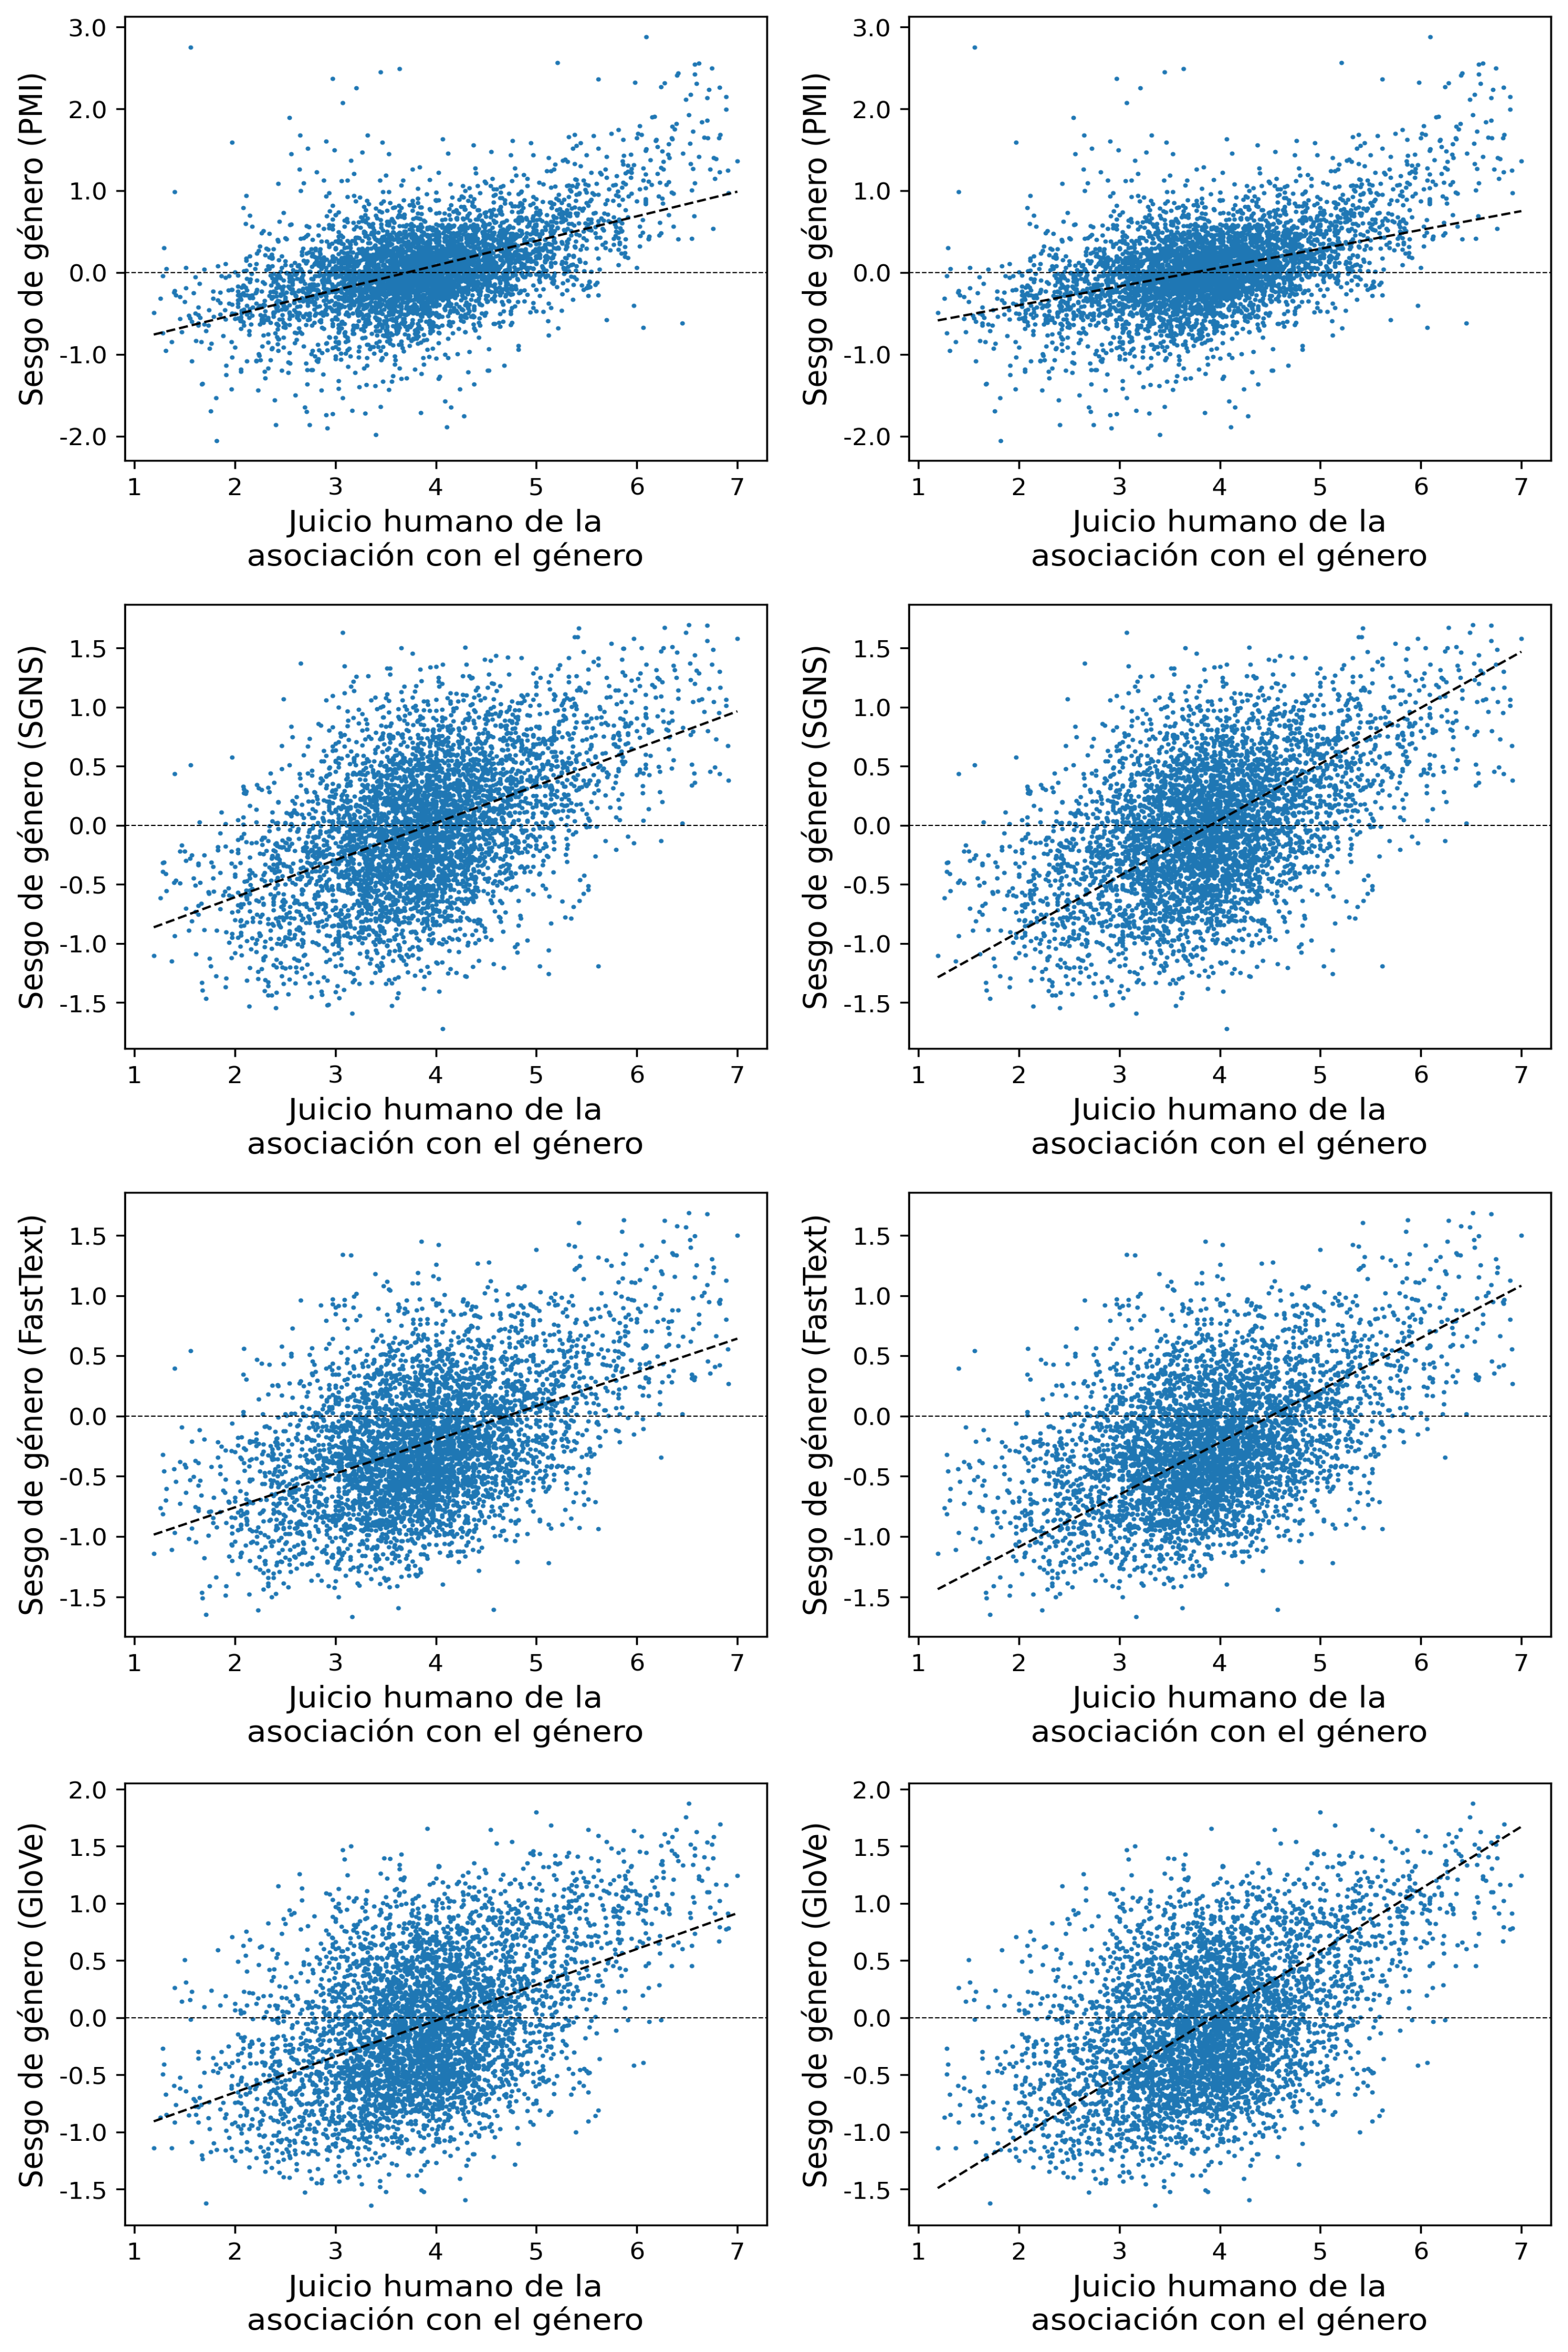
\includegraphics[width=0.85\textwidth]{img/grid_glasgow-gender.png}
    \caption{
        Relación entre el sesgo de género textual y de acuerdo al juicio humano en las palabras de \citet{lewis2020gender}. Cada punto representa una palabra objetivo. Las rectas representan un ajuste lineal de los datos. En la segunda fila el ajuste pondera cada punto por el error estándar de la estimación de sesgo textual (los intervalos de confianza asociados no se muestran para mayor claridad).
    }
    \label{fig:grid_corr_genero}
\end{figure}

\begin{figure}[H]
    \centering
    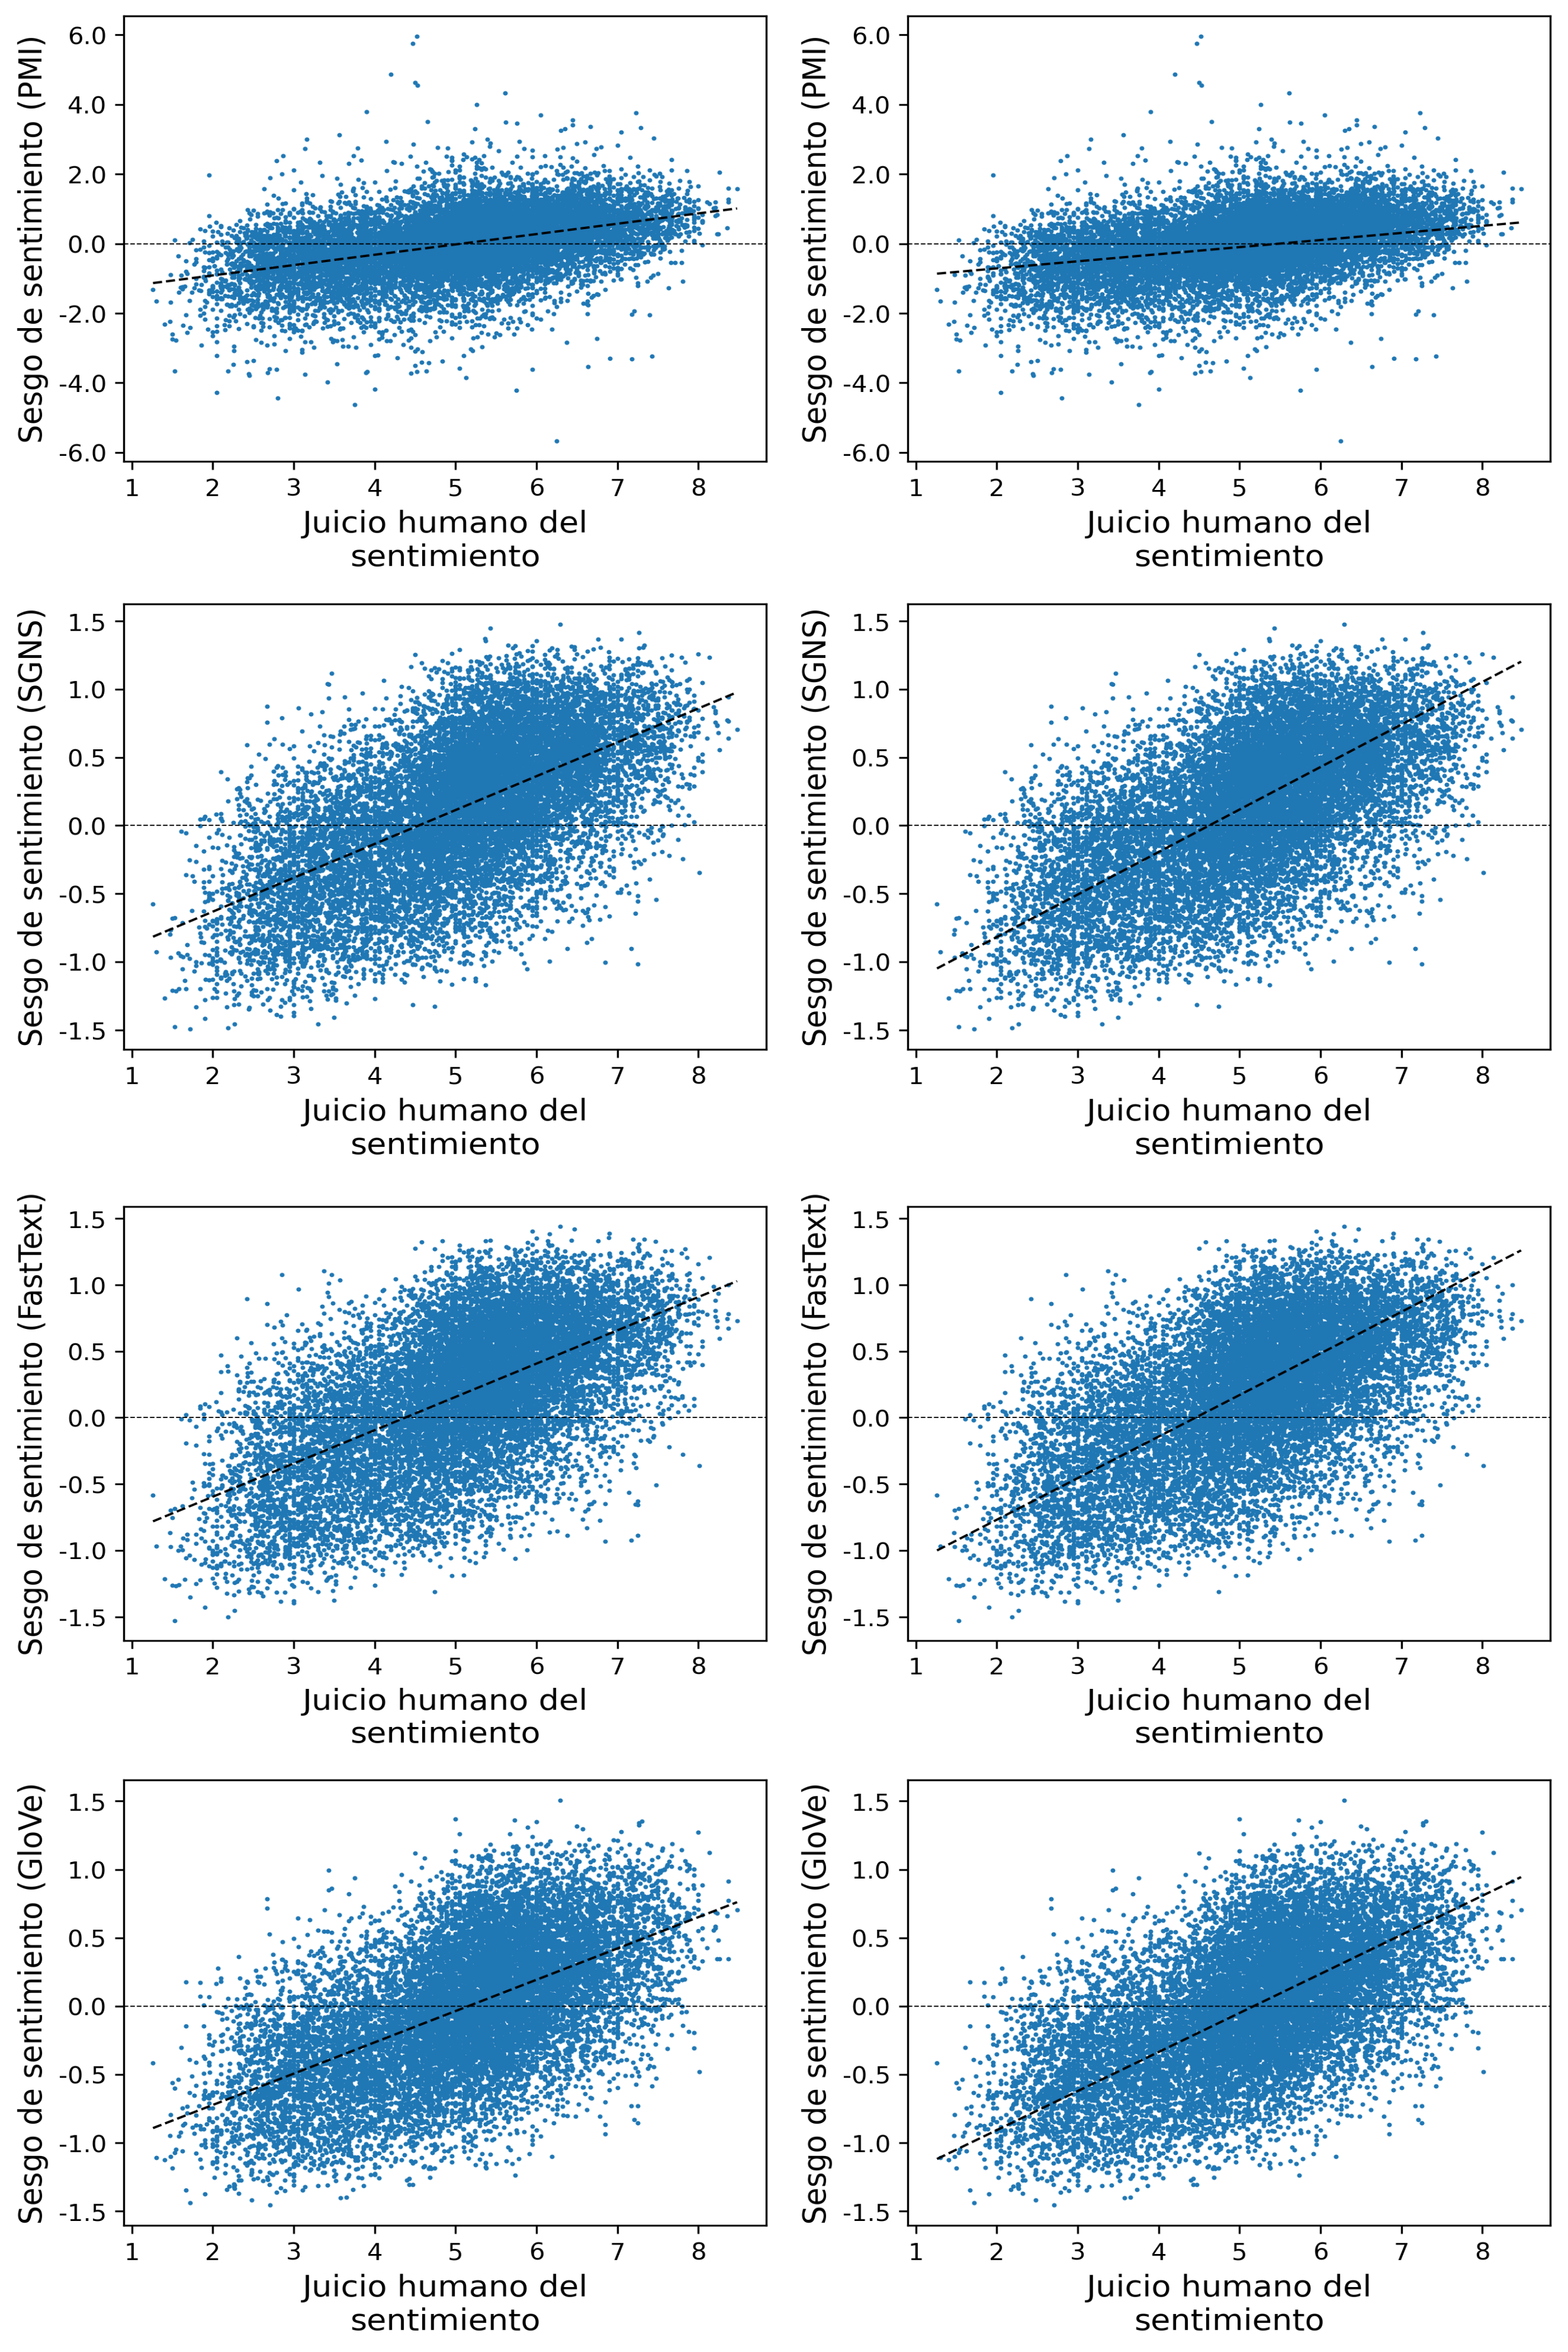
\includegraphics[width=0.85\textwidth]{img/grid_warriner-valence.png}
    \caption{
        Relación entre el sesgo de sentimiento textual y de acuerdo al juicio humano en las palabras de \citet{toney2021valnorm}. Cada punto representa una palabra objetivo. Las rectas representan un ajuste lineal de los datos. En la segunda fila el ajuste pondera cada punto por el error estándar de la estimación de sesgo textual (los intervalos de confianza asociados no se muestran para mayor claridad).
    }
    \label{fig:grid_corr_sentimiento}
\end{figure}

\begin{figure}[H]
    \centering
    \includegraphics[width=0.85\textwidth]{img/grid_mturk-race.png}
    \caption{
        Relación entre el sesgo étnico textual y de acuerdo al juicio humano en las palabras de \citet{kozlowski2019geometry}. Cada punto representa una palabra objetivo. Las rectas representan un ajuste lineal de los datos. En la segunda fila el ajuste pondera cada punto por el error estándar de la estimación de sesgo textual (los intervalos de confianza se indican con barras de error).
    }
    \label{fig:grid_corr_etnico}
\end{figure}


Encontramos \textbf{correlaciones positivas entre todas las métricas de sesgo textual y los sesgos de acuerdo al juicio humano} (ver la Tabla \ref{tab:correlaciones} con los coeficientes de correlación; los diagramas de dispersión asociados se encuentran en las Figuras \ref{fig:grid_corr_genero}, \ref{fig:grid_corr_sentimiento} y \ref{fig:grid_corr_etnico}). Esto es consistente con los hallazgos previos de los estudios en los cuales están basados los tres experimentos \citep{lewis2020gender,kozlowski2019geometry,toney2021valnorm}, los cuales usan métricas de sesgo textual basadas en \emph{word embeddings}.

También hallamos que, en general, el uso de ponderadores para calcular la correlación aumenta los coeficientes de $\BiasWE$. Esto implica que reducir la ponderación de estimaciones más ruidosas (donde la diferencia de similitudes con respecto a las listas de palabras $A$ y $B$ no es tan sistemática) tiende a incrementar la correlación del sesgo de este \emph{corpus}. En cambio, los coeficientes de correlación de $\BiasPMI$ tienden a caer o permanecer constantes cuando se usan ponderadores, lo cual indica que los pesos tienden a ser mayores en palabras donde el sesgo textual estimado no coincide con el sesgo de acuerdo al juicio humano. No tenemos ninguna hipótesis sobre por qué el efecto de usar ponderadores es distinto para $\BiasWE$ y $\BiasPMI$.

Remarcamos que esto no significa que para cada estimación individual de sesgo los errores estándar de cada método sean mutuamente intercambiables o igualmente útiles, dado que capturan tipos de variabilidad distinta (ver secciones \ref{sec:bias_pmi_variabilidad} y \ref{sec:experimento_variabilidad}). Esto se ve reflejado en que los intervalos de confianza de $\BiasWE$ tienden a ser relativamente más anchos en $\BiasWE$ que en $\BiasPMI$, como se observa en la Figura \ref{fig:grid_corr_etnico}. 

Tomando como referencia el coeficiente de correlación más alto de cada tipo de métrica ($\BiasPMI$ vs. $\BiasWE$) en cada sesgo, se obtienen correlaciones más altas con $\BiasWE$ que con $\BiasPMI$. La diferencia es particularmente alta en el caso del sesgo étnico ($\max(r_{\BiasWE})=0.51$ vs. $\max(r_{\BiasPMI})=0.15$), donde además el grado de correlación de $\BiasPMI$ es especialmente débil. 

Una hipótesis que puede explicar este resultado es que en este estereotipo las \textbf{asociaciones de segundo orden} juegan un rol importante, y éstas no son capturadas por $\BiasPMI$. Determinados consumos culturales como el \emph{basketball} pueden estar más asociados a \emph{black} que a \emph{white} no porque \emph{basketball} aparezca relativamente más en el contexto de palabras que explícitamente refieren a \emph{black} (las palabras de contexto), sino porque comparten vecinos en común, como pueden ser los nombres de las personas que juegan al basketball.

Este tipo de asociación puede ser capturada por los puntajes de juicio humano y por $\BiasWE$, pero no necesariamente por $\BiasPMI$. Una manera de capturar esto con $\BiasPMI$ puede ser extendiendo las listas de palabras de contexto, por ejemplo con nombres propios o apellidos típicos de cada etnia (como se realiza, por ejemplo, en \citet{garg2018word}). En la sección \ref{sec:experimento_interpretabilidad} discutimos con mayor detalle las diferencias entre $\BiasPMI$ y $\BiasWE$ en términos de los tipos de asocaciones semánticos y aspectos del \emph{corpus} que capturan.  

Enfatizamos que no consideramos que los coeficientes de correlación con el juicio humano (Tabla \ref{tab:correlaciones}) sean una medida de la bondad global de una métrica de sesgo. El objetivo de nuestro análisis es analizar en qué medida los resultados que se obtienen con los dos tipos de métricas son similares. Con otras listas de palabras probablemente se obtengan otros resultados. Asimismo, es probable que Wikipedia no sea necesariamente representativa de los estereotipos sociales codificados en los puntajes de las encuestas que se usan en cada experimento. Incorporar \emph{corpora} de otros dominios podría dar lugar a correlaciones mayores o menores. 

Por otra parte, hasta donde sabemos, no existen \emph{corpora} anotados con los sesgos que contienen. Disponer de ese \emph{ground truth} sería valioso para la tarea de medir sesgos en textos porque permitiría evaluar las métricas de manera más directa, comparando el sesgo textual estimado con el sesgo anotado. Sin embargo, no es obvio cómo anotar la cantidad de sesgo de una palabra en un \emph{corpus}, particularmente si el \emph{corpus} es grande. En los tres experimentos que estudiamos, las ``anotaciones'' son promedios de valoraciones de humanos sobre la semántica de las palabras, y no tienen en cuenta ningún \emph{corpus} en particular. La falta de estas etiquetas hace que no esté claro cómo sacar conclusiones sobre si un método es globalmente mejor que otro a la hora de medir el sesgo en palabras específicas de un texto.


\section{Interpretación de las estimaciones} \label{sec:experimento_interpretabilidad}

En esta sección, analizamos las ventajas y desventajas de medir los sesgos con \emph{word embeddings} en comparación a una métrica de asociación de primer orden como $\BiasPMI$. En particular, usaremos ejemplos concretos de mediciones de sesgo de género binario para \textbf{comparar la interpretación de las estimaciones con cada método}.

Como hemos visto en la sección \ref{sec:bias_pmi}, $\BiasPMI$ puede expresarse intrínsecamente en términos de probabilidades condicionales (ecuación \ref{eq:bias_pmi_condicional}). El sesgo se interpreta en este caso como el logaritmo de cuánto más probable es encontrar palabras de $C$ en el contexto de palabras en $A$ que en el contexto de palabras en $B$. Dado que \textbf{$\BiasPMI$ puede interpretarse de forma transparente en términos de coocurrencias de primer orden}, podemos decir que $\BiasPMI$ es una métrica absoluta que no requiere comparaciones con otros sesgos para ser interpretada. 

Podemos ilustrar esta propiedad con un ejemplo individual. Cuando medimos el sesgo de género binario (femenino/masculino) en el \emph{corpus} de Wikipedia, obtenemos que $\BiasPMI(nurse)$ $\approxeq
1,3172$. Por lo tanto,
%
\begin{equation*}
    \frac{P(nurse|A)}{P(nurse|B)} \approxeq
    e^{1,3172} \approxeq
    3,7330.
\end{equation*}
%
Esto significa que es aproximadamente un 273,30 \% más probable encontrar la palabra \emph{nurse} en el contexto de palabras femeninas ($A$) que en el contexto de palabras masculinas ($B$).

En el caso de $\BiasWE$, si bien existen estudios que buscan interpretar cómo se forman los espacios vectoriales de los \emph{embeddings} \citep{levy2014neural,levy2015improving,ethayarajh2019understanding} o que analizan los patrones semánticos que codifican \citep{bolukbasi2016man,zhao2017men,gonen2019lipstick}, no existe una interpretación transparente de las métricas de sesgo basadas en \emph{embeddings} en términos de las coocurrencias de palabras en los textos.

Esta falta de interpretabilidad de $\BiasWE$ se debe a que la similitud entre \emph{embeddings} como SGNS, GloVe y FastText puede captar asociaciones entre palabras tanto de primer orden (sintagmáticas) como de segundo orden (paradigmáticas) o superior \citep{altszyler2018corpus,schlechtweg2019second}. Entonces, cuando usamos \emph{embeddings} para medir sesgos, no es posible saber si los resultados se deben a coocurrencias de primer orden generalizadas o se derivan de coocurrencias de orden superior poco transparentes \citep{brunet2019understanding,rekabsaz2021measuring}. En definitiva, mientras \textbf{la relación entre $\BiasWE$ y la distribución de palabras no es transparente}, en el caso de $\BiasPMI$ sí lo es porque $\PMI$ es estrictamente una métrica de asociación de primer orden.

% NOTE estos valores en realidad son de OpenSubs pero puse Wiki porque no usé OpenSubs en la tesis (:

Ejemplificamos esta diferencia en interpretabilidad con el caso de la palabra \emph{evil}. En Wikipedia, el $\BiasPMI$ de género de \emph{evil} es igual a $-0,25$, lo que indica una mayor probabilidad de aparecer en el contexto de palabras de contexto masculino ($B$) en comparación con las femeninas ($A$). Por el contrario, $\BiasWE=0,23$ con SGNS. Aunque sabemos que esto se interpreta como un sesgo femenino, es difícil comprender el origen exacto de este resultado porque está influido por coocurrencias de segundo orden o superior, y no podemos medir el peso que tiene cada uno de estos factores. 

A continuación mostramos otros ejemplos que ilustran cómo el orden de asociación puede influir en las estimaciones de sesgo de género:

\begin{itemize}

    % NOTE estos valores en realidad son de OpenSubs pero puse Wiki porque no usé OpenSubs en la tesis (:
    \item Hay palabras no incluidas en el grupo $A$ que intrínsecamente tienen un sesgo femenino, como \emph{women}, \emph{wife}, \emph{ladies} o \emph{girls}. Sin embargo, estas palabras aparecen con $\BiasPMI < 0$ (sesgo masculino) porque tienden a aparecer relativamente más en el contexto de palabras masculinas (grupo $B$) que femeninas (grupo $A$) en Wikipedia (por ejemplo, \emph{his wife}). Probablemente la asociación de estas palabras con las del grupo $A$ sea de segundo orden o paradigmática (tienden a tener vecinos similares), y este aspecto no es capturado por $\BiasPMI$.
    
    % NOTE estos valores en realidad son de OpenSubs pero puse Wiki porque no usé OpenSubs en la tesis (:
    \item Ocupaciones como \emph{assistant} y \emph{secretary} están estereotípicamente asociadas al género femenino \citep{caliskan2017semantics}. Sin embargo, obtenemos valores de $\BiasPMI$ de género de $-0,19$ y $-0,24$,  respectivamente (ambos con p-valor $< 10^{-5}$). Esto indica una asociación de primer orden más fuerte con las palabras de contexto masculinas ($B$) en comparación con las femeninas ($A$); por ejemplo, por la presencia de estructuras como \emph{his assistant}. Al usar $\BiasWE$ con SGNS obtenemos valores de $0,70$ y $0,43$, respectivamente: el sesgo invierte su signo. Esto podría deberse al efecto de la asociación de segundo orden: estas palabras probablemente tienen vecinos similares a las palabras del grupo $A$, es decir, aparecen en contextos similares (por ejemplo, contextos relacionados a la oficina o el cuidado).
    
    % NOTE esto sí es de wiki:
    \item Palabras como \emph{harbor}, \emph{navy}, \emph{dock}, \emph{port}, \emph{fleet}, \emph{steam}, \emph{pier}, \emph{sailor}, \emph{ship}, y \emph{sail} tienen valores positivos de $\BiasPMI$ de género en Wikipedia. Esto puede deberse a que en el idioma inglés, los barcos se suelen denominar con pronombres femeninos como \emph{she}. Los valores de $\BiasWE$ con SGNS para estas palabras son, en cambio, inferiores a 0, posiblemente porque estas palabras están más relacionadas con el género masculino a través de coocurrencias de segundo orden (e.g. los barcos y los varones pueden aparecer en contextos similares relacionados a la marina o la guerra).

\end{itemize}

Otro aspecto interesate a considerar es que las métricas de sesgo que capturan asociaciones de segundo orden tienen la ventaja de \textbf{gestionar la \emph{raleza} de los datos (\emph{data sparsity})}. Dado que todo \emph{corpus} es limitado, algunas de las muchas formas que pueden tomar los conceptos objetivo y de contexto pueden aparecer raramente en el texto. En este escenario en el que las coocurrencias son ralas (\emph{sparse}), cuando usamos $\BiasWE$, puede que no sea necesario incluir todas las palabras relacionadas con los conceptos objetivo y de contexto para medir sesgos exitosamente, dado que los \emph{embeddings} pueden captar sinonimia. En el caso de $\BiasPMI$, este problema debe abordarse aumentando las listas de palabras con sinónimos y formas de las palabras de interés.

Para ejemplificar esto, consideremos el caso de los sinónimos \emph{nourish} y \emph{nurture}, que tienen frecuencias diferentes en el corpus de Wikipedia ($700$ y $3,000$, respectivamente). Con $\BiasPMI$, obtenemos un sesgo de $0,33$ para \emph{nurture} (p-valor $< 10^{-4}$). Sin embargo, si hubiéramos utilizado en su lugar su sinónimo menos frecuente \emph{nourish}, el $\BiasPMI$ habría sido $-0,10$ y no habría sido estadísticamente significativo (p-valor $\approx 0,66$). En este caso no habríamos podido determinar si realmente no hay sesgo o si la cantidad de datos es insuficiente para determinar esto. 

Esto demuestra que, en general, es aconsejable incluir todos los sinónimos y variaciones pertinentes del término cuyo sesgo intentamos medir cuando usamos $\BiasPMI$. Por otra parte, cuando se usa $\BiasWE$ podríamos confiar en el hecho de que los \emph{embeddings} pueden capturar sinonimia; en este ejemplo particular $\BiasWE$ con SGNS arroja valores positivos para ambas palabras.

Por último, en investigaciones recientes hemos demostrado que \textbf{$\BiasWE$, a diferencia de $\BiasPMI$, puede producir resultados engañosos porque captura inadvertidamente las disparidades en las frecuencias de las palabras de contexto} \citep{valentini2022undesirable}. 

Para dar cuenta de este problema en el contexto de la interpretabilidad, analizamos las estimaciones de sesgo de \emph{stopwords}, es decir, palabras muy frecuentes con poco contenido semántico (ver Tabla \ref{tab:stopwords}). Mientras que $\BiasPMI$ no tiende a detectar sesgo de género sistemáticamente en alguna dirección en las \emph{stopwords}, $\BiasWE$ con cualquiera de los tres métodos de generación de \emph{embeddings} tiende a producir estimaciones de sesgo siempre negativas i.e. con sesgo masculino. Esto se debe a que las palabras de contexto masculinas (grupo $B$) son más frecuentes que las femeninas (grupo $A$) en el corpus de Wikipedia, y a que los \emph{embeddings} tienen la capacidad de capturar la frecuencia de las palabras \citep
{valentini2022undesirable}. 



\begin{table}[h]
  \centering
  \begin{tabular}{lrrrr}
    \toprule
    Palabra & PMI   & SGNS  & FastText & GloVe \\
    \midrule
    which   & -0.08 & -0.50 & -0.59    & -0.51 \\
    first   & 0.03  & -0.15 & -0.28    & -0.50 \\
    after   & -0.06 & -0.60 & -0.73    & -0.62 \\
    have    & 0.13  & -0.42 & -0.35    & -0.45 \\
    other   & 0.07  & -0.57 & -0.45    & -0.44 \\
    all     & -0.05 & -0.55 & -0.58    & -0.64 \\
    over    & -0.20 & -0.80 & -0.87    & -0.76 \\
    only    & 0.02  & -0.46 & -0.56    & -0.60 \\
    most    & -0.13 & -0.53 & -0.56    & -0.62 \\
    up      & 0.11  & -0.63 & -0.67    & -0.64 \\
    used    & -0.13 & -0.72 & -0.38    & -0.68 \\
    under   & -0.16 & -0.96 & -1.12    & -1.15 \\
    part    & 0.07  & -0.31 & -0.41    & -0.40 \\
    many    & -0.15 & -0.42 & -0.60    & -0.64 \\
    well    & 0.04  & -0.29 & -0.44    & -0.52 \\
    name    & 0.13  & -0.26 & -0.28    & -0.50 \\
    several & -0.09 & -0.36 & -0.53    & -0.53 \\
    same    & 0.05  & -0.06 & -0.40    & -0.54 \\
    former  & -0.21 & -0.60 & -0.59    & -0.59 \\
    system  & -0.55 & -1.01 & -0.77    & -0.93 \\
    \bottomrule
  \end{tabular}
  \caption{
    Sesgo de género de las 20 \emph{stopwords} más frecuentes de las palabras del experimento de Glasgow \citep{scott2019glasgow}.
  }
  \label{tab:stopwords}
\end{table}



En consecuencia, no podemos interpretar qué aspectos del corpus dan lugar a las estimaciones de sesgo que observamos. Cuando usamos $\BiasWE$, en definitiva, no solo es dificil determinar el tipo de asociación que da origen a los resultados, sino también si el sesgo semántico detectado es genuino o si sólo se debe a la disparidad en las frecuencias de las palabras de contexto.

